\chapter{Algorytmy grupowania gęstościowego}

Istniejące algorytmu grupowania można podzielić ze względu na to jak definiują pojęcie grupy. Jedną z klas algorytmów grupowania są właśnie algorytmy grupowania gęstościowego. Jak wskazuje nazwa, grupy określa się na podstawie lokalnej gęstości punktów, co zgadza się z intuicyjnym pojęciem grupy.\par

Część algorytmów grupowania gęstościowego opiera się na dzieleniu przestrzeni na siatkę komórek, gdzie grupy określane są na podstawie uśrednionej gęstości wewnątrz tychże komórek. O ile takie podejście jest proste i wydajne, to nie jest dokładne, a wyniki grupowania mogą zależeć od rozmieszczenia siatki. Algorytm DBSCAN reprezentuje podejście, które rozwiązuje te problemy. Przynależność do grupy jest rozstrzygana dla każdego punktu oddzielnie, więc grupowanie jest dokładne co do punktu. Co więcej, wyniki są deterministyczne z dokładnością do tak zwanych punktów brzegowych.\par
Definicja grupy zaproponowana w DBSCAN okazała się na tyle skuteczna, że powstały liczne algorytmy pochodne opierające się na tej samej lub podobnej definicji grupy. Takimi algorytmami są SUBCLU oraz PREDECON. Obydwa należą do klasy algorytmów grupowania w podprzestrzeniach, co oznacza, że są w stanie wyznaczać grupy w podzbiorach atrybutów grupowanych obiektów.\par
W tym rozdziale zostaną przedstawione trzy wspomniane wcześniej algorytmy: DBSCAN, SUBCLU oraz PREDECON.


Istniejące algorytmu grupowania można podzielić ze względu na to jak definiują pojęcie grupy. Jedną z klas algorytmów grupowania są właśnie algorytmy grupowania gęstościowego. Jak wskazuje nazwa, grupy określa się na podstawie lokalnej gęstości punktów, co zgadza się z intuicyjnym pojęciem grupy.\par

Część algorytmów grupowania gęstościowego opiera się na dzieleniu przestrzeni na siatkę komórek, gdzie grupy określane są na podstawie uśrednionej gęstości wewnątrz tychże komórek. O ile takie podejście jest proste i wydajne, to nie jest dokładne, a wyniki grupowania mogą zależeć od rozmieszczenia siatki. Algorytm DBSCAN reprezentuje podejście, które rozwiązuje te problemy. Przynależność do grupy jest rozstrzygana dla każdego punktu oddzielnie, więc grupowanie jest dokładne co do punktu. Co więcej, wyniki są deterministyczne z dokładnością do tak zwanych punktów brzegowych.\par
Definicja grupy zaproponowana w DBSCAN okazała się na tyle skuteczna, że powstały liczne algorytmy pochodne opierające się na tej samej lub podobnej definicji grupy. Takimi algorytmami są SUBCLU oraz PREDECON. Obydwa należą do klasy algorytmów grupowania w podprzestrzeniach, co oznacza, że są w stanie wyznaczać grupy w podzbiorach atrybutów grupowanych obiektów.\par
W tym rozdziale zostaną przedstawione trzy wspomniane wcześniej algorytmy: DBSCAN, SUBCLU oraz PREDECON.

\section{DBSCAN}
DBSCAN jest popularnym algorytmem grupowania gęstościowego. Najważniejsze jego zalety wymienione w \cite{dbscan} to tworzenie grup o dowolnym kształcie oraz możliwość doboru parametrów przy niewielkiej wiedzy o zbiorze danych. Grupy tworzone są na podstawie lokalnej gęstości punktu rozumianej jako liczba punktów w otoczeniu punktu, dzięki czemu tworzone są grupy o intuicyjnych kształtach.

Zakładamy, że grupowany jest zbiór punktów $ D $. Na potrzebę algorytmu definiuje się pojęcie $ \varepsilon $-otoczenia punktu $ p \in D $. Jest to zbiór punktów znajdujących się w odległości nie większej niż punkt, dla którego jest wyznaczane otoczenie. Dalej $ \varepsilon $-otoczenie punktu $ p $ będzie oznaczane $ N_\varepsilon(p) $.
\begin{equation}\label{eps-neighbourhood}
	N_\varepsilon(p) = \set{q \in D | d(p, q) \le \varepsilon}
\end{equation}

Punkt, który posiada w swoim otoczeniu $ N_\varepsilon(p) $ conajmniej $ \mu $ punktów jest nazywany punktem rdzeniowym.
\begin{equation}\label{core-point}
	core_{\varepsilon,\mu}(p) \iff |N_\varepsilon(p)| \le \mu
\end{equation}
\begin{figure}
	\centering
  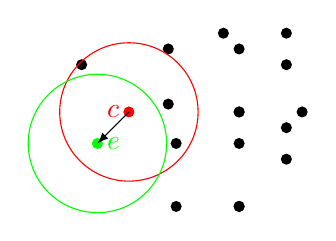
\begin{tikzpicture}
		\fill (-2,1.8) circle(2pt);
		\fill (-.9, 1.3) circle(2pt);
		\fill (-.9,2) circle(2pt);
		\fill (-.8,.8) circle(2pt);
		\fill (-.8,0) circle(2pt);
		\fill (-.2,2.2) circle(2pt);
		\fill (0,0) circle(2pt);
		\fill (0,1.2) circle(2pt);
		\fill (0,1.2) circle(2pt);
		\fill (0,0) circle(2pt);
		\fill (0,.8) circle(2pt);
		\fill (0,2) circle(2pt);
		\fill (.6,1) circle(2pt);
		\fill (.6,.6) circle(2pt);
		\fill (.6,1.8) circle(2pt);
		\fill (.6,2.2) circle(2pt);
		\fill (.8,1.2) circle(2pt);
    
    \fill[red] (-1.4,1.2) circle(2pt) node[anchor=east]{$ c $};
    \draw[red] (-1.4,1.2) circle(25pt);
    
    \fill[green] (-1.8,.8) circle(2pt) node[anchor=west]{$ e $};
    \draw[green] (-1.8,.8) circle(25pt);
    
		\draw[-latex] (-1.4,1.2) -- (-1.8,.8);
		
  \end{tikzpicture}
  \caption{Punkt rdzeniowy $ c $, brzegowy $ e $ oraz relacja bezpośredniej gęstościowej osiągalności $ dirreach_{\varepsilon,\mu}(e, c) $, $ \mu=3$.}\label{fig:core-edge-point}
\end{figure}

Dalej, na potrzebę definicji grupy wprowadza się pojęcie bezpośredniego zasięgu gęstościowego. Jest to niesymetryczna relacja, która zachodzi jeśli punkt znajduje się w $ \varepsilon $-otoczeniu punktu rdzeniowego. Punkt $ p $ jest w bezpośrednim zasięgu gęstościowym punktu $ q $, jeśli punkt $ q $ jest punktem rdzeniowym i $ p $ znajduje się w $ \varepsilon $-otoczeniu punktu $ q $.
\begin{equation} \label{direct-reachability}
	dirreach_{\varepsilon,\mu}(p, q) \iff p \in N_\varepsilon(q) \land core_{\varepsilon,\mu}(q)
\end{equation}
To, że $ p $ jest w bezpośrednim zasięgu gestościowym $ q $ nie determinuje, \mbox{że $ q $ jest} w bezpośrednim zasięgu gęstościowym $ p $.
\begin{equation} \label{direct-reachability-asymmetry}
	dirreach_{\varepsilon,\mu}(p, q) \centernot \implies dirreach_{\varepsilon,\mu}(q, p)
\end{equation}

Punkt, który jest w bezpośrednim zasięgu gęstościowym innego punktu, ale sam nie jest punktem rdzeniowym jest nazywany punktem brzegowym.
\begin{equation}\label{edge-point}
	edge_{\varepsilon,\mu}(p) \iff \neg core_{\varepsilon,\mu}(p) \land dirreach_{\varepsilon,\mu}(p,q)
\end{equation}

Jeśli punkt $ p $ jest w bezpośrednim zasięgu gęstościowym $ q $, to jest też w zasięgu gęstościowym $ q $. 
\begin{equation}
	dirreach_{\varepsilon,\mu}(p, q) \implies reach_{\varepsilon,\mu}(p, q)
\end{equation}
Zasięg gęstościowy jest relacją przechodnią, to znaczy, że jeśli $ p $ jest w zasięgu gęstościowym $ q $  i $ q $ jest w zasięgu gęstościowym $ r $, to $ p $ jest też w zasięgu gęstościowym $ r $.
\begin{equation}
	reach_{\varepsilon,\mu}(p, q) \land reach_{\varepsilon,\mu}(q, r) \implies reach_{\varepsilon,\mu}(p, r)
\end{equation}
Podobnie jak relacja bezpośredniego zasięgu gęstościowego, zasięg gęstościowy nie jest symetryczny.
\begin{equation}
	reach_{\varepsilon,\mu}(p, q) \centernot \implies reach_{\varepsilon,\mu}(q, p)
\end{equation}

Dwa punkty są gęstościowo połączone jeśli istnieje taki punkt, że obydwa są w jego zasięgu gęstościowym.
\begin{equation}
	reach_{\varepsilon,\mu}(p, q) \land reach_{\varepsilon,\mu}(p, r) \implies connected_{\varepsilon,\mu}(q, r)
\end{equation}
Łączność gęstościowa jest relacją symetryczną i przechodnią. Jeśli dwa punkty są gęstościowo połączone, to należą do tej samej grupy. Grupę można zdefiniować jako maksymalny zbiór punktów połączonych gęstościowo.
\begin{equation}
	\begin{cases} 
		\forall p, q \in C\,connected_{\varepsilon,\mu}(p,q) \\
		r \notin C \implies \forall s \in C \,\neg connected_{\varepsilon,\mu}(r, s)
	\end{cases}
\end{equation}
\begin{figure}
	\begin{minipage}[b]{.5\linewidth}
		\centering
		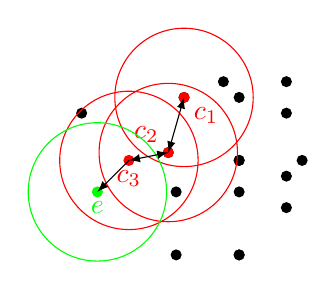
\begin{tikzpicture}
			\fill (-2,1.8) circle(2pt);
			\fill (-.9, 1.3) circle(2pt);
			\fill (-.8,.8) circle(2pt);
			\fill (-.8,0) circle(2pt);
			\fill (-.7,2) circle(2pt);
			\fill (-.2,2.2) circle(2pt);
			\fill (0,0) circle(2pt);
			\fill (0,1.2) circle(2pt);
			\fill (0,1.2) circle(2pt);
			\fill (0,0) circle(2pt);
			\fill (0,.8) circle(2pt);
			\fill (0,2) circle(2pt);
			\fill (.6,1) circle(2pt);
			\fill (.6,.6) circle(2pt);
			\fill (.6,1.8) circle(2pt);
			\fill (.6,2.2) circle(2pt);
			\fill (.8,1.2) circle(2pt);
			
			\fill[red] (-.7, 2) circle(2pt) node[anchor=north west]{$ c_1 $};
			\draw[red] (-.7, 2) circle(25pt);
			
			\fill[red] (-.9, 1.3) circle(2pt) node[anchor=south east]{$ c_2 $};
			\draw[red] (-.9, 1.3) circle(25pt);
			
			\fill[red] (-1.4,1.2) circle(2pt) node[anchor=north]{$ c_3 $};
			\draw[red] (-1.4,1.2) circle(25pt);
			
			\fill[green] (-1.8,.8) circle(2pt) node[anchor=north]{$ e $};
			\draw[green] (-1.8,.8) circle(25pt);
			
			\draw[latex-latex] (-.7, 2) -- (-.9, 1.3);
			\draw[latex-latex] (-.9, 1.3) -- (-1.4,1.2);
			\draw[-latex] (-1.4,1.2) -- (-1.8,.8);
		\end{tikzpicture}
		\subcaption{$ reach_{\varepsilon,\mu}(e, c_1) $} \label{fig:density-reachablity-reachability}
	\end{minipage}
	\begin{minipage}[b]{.5\linewidth}
		\centering
		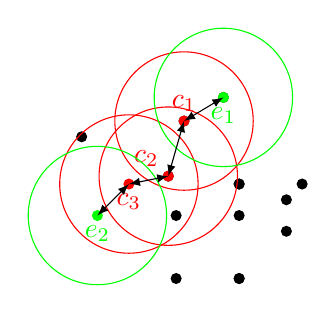
\begin{tikzpicture}
			\fill (-2,1.8) circle(2pt);
			\fill (-.9, 1.3) circle(2pt);
			\fill (-.8,.8) circle(2pt);
			\fill (-.8,0) circle(2pt);
			\fill (-.7,2) circle(2pt);
			\fill (-.2,2.3) circle(2pt);
			\fill (0,0) circle(2pt);
			\fill (0,1.2) circle(2pt);
			\fill (0,1.2) circle(2pt);
			\fill (0,0) circle(2pt);
			\fill (0,.8) circle(2pt);
			\fill (.6,1) circle(2pt);
			\fill (.6,.6) circle(2pt);
			\fill (.8,1.2) circle(2pt);
			
			\fill[red] (-.7, 2) circle(2pt) node[anchor=south]{$ c_1 $};
			\draw[red] (-.7, 2) circle(25pt);
			
			\fill[red] (-.9, 1.3) circle(2pt) node[anchor=south east]{$ c_2 $};
			\draw[red] (-.9, 1.3) circle(25pt);
			
			\fill[red] (-1.4,1.2) circle(2pt) node[anchor=north]{$ c_3 $};
			\draw[red] (-1.4,1.2) circle(25pt);
			
			\fill[green] (-1.8,.8) circle(2pt) node[anchor=north]{$ e_2 $};
			\draw[green] (-1.8,.8) circle(25pt);
			
			\fill[green] (-.2,2.3) circle(2pt) node[anchor=north]{$ e_1 $};
			\draw[green] (-.2,2.3) circle(25pt);
			
			\draw[latex-latex] (-.2,2.3) -- (-.7, 2);
			\draw[latex-latex] (-.7, 2) -- (-.9, 1.3);
			\draw[latex-latex] (-.9, 1.3) -- (-1.4,1.2);
			\draw[latex-latex] (-1.4,1.2) -- (-1.8,.8);
		\end{tikzpicture}
		\subcaption{$ connected_{\varepsilon,\mu}(e_1, e_2) $} \label{fig:density-reachablity-connection}
	\end{minipage}
	\caption{Relacje gęstościowej osiągalności \subref{fig:density-reachablity-reachability} oraz łączności \mbox{gęstościowej \subref{fig:density-reachablity-connection},} $ \mu = 3 $.}
\end{figure}

Punkty, które nie należą do żadnej z grup nazywa się szumem. Takie punkty nie są gęstościowo połączone z żadnym innym punktem.
\begin{equation}
	noise_{\varepsilon,\mu}(p) \iff \forall i \,p\notin C_i \iff \forall q \in D \,\neg connected(p,q)
\end{equation}

\begin{algorithm}
 	\caption{DBSCAN \cite{dbscan}}\label{alg:dbscan}

	\DontPrintSemicolon
	
	\SetKwFunction{dbscan}{dbscan}
	\SetKwFunction{expand}{expandcluster}
	
	\setcounter{AlgoLine}{0}
	\nonl\SetKwProg{myproc}{Wejście}{}{}
	\myproc{}{
		$D$ - zbiór danych \;
		$\varepsilon $ - promień otoczenia \;
		$\mu $ - próg liczności otoczenia \;
	}
	\setcounter{AlgoLine}{0}
	\nonl\SetKwProg{myproc}{Wyjście}{}{}
	\myproc{}{
		każdy punkt zbioru $ D $ ma przypisaną etykietę grupy lub szumu\;
	}
	
	
	\setcounter{AlgoLine}{0}
	\nonl\SetKwProg{myproc}{Definicje}{}{}
	\myproc{}{
		$ nextcid() $ - zwraca nową unikalną etykietę grupy\;
		$ noise $ - etykieta szumu\;
		$ unde\f{}ined $ - nieokreślona etykieta\;
		$ cid(v) $ - etykieta punktu $ v $\;
		$ N_{V,\varepsilon}(v) $ - $ \varepsilon $-otoczenie punktu $ v $ w zbiorze $ V $ (\myhyperref{eps-neighbourhood}{wyrażenie})\;
		$ any(V) $ - dowolny element zbioru $ V $\;
		$ core_{V,\varepsilon,\mu}(v) $ - $ v $ jest punktem rdzeniowym w $ V $(\myhyperref{core-point}{wyrażenie})\;
	}
	\nonl\SetKwProg{myalg}{Algorytm}{}{}
	\myalg{\dbscan{$D$, $\varepsilon$, $\mu$}}{
		$ cid \gets nextcid() \;$ \tcp*{etykieta grupy}
		\ForEach{v \textbf{in} D}{
			\If{$ cid(v) = unde\f{}ined $}{
				\lIf{\expand{D, v, cid, $ \varepsilon $, $ \mu $}}{
					$ cid \gets nextcid() $
				}
			}
		}
	}
	\setcounter{AlgoLine}{0}
	\nonl\SetKwProg{myproc}{Procedura}{}{}
	\myproc{\expand{D, v, cid, $ \varepsilon $, $ \mu $}}{
		$ N_v \gets N_{D,\varepsilon}(v) $\;
		\uIf(\tcp*[f]{$ core_{D,\varepsilon,\mu}(v) $}){$ |N_v| \ge \mu $}{ 
			$ seeds \gets \set{w \in N_v | cid(w) = unde\f{}ined \land w \neq v} $\;
			\lForEach{$ w\ \mathbf{in}\ N_v $}{$ cid(w) \gets cid $}
			\While{$ seeds \neq \emptyset $} {
				$ w \gets any(seeds) $\;
				$ seeds \gets seeds \setminus \set{w} $\;
				$ N_w \gets N_{D,\varepsilon}(w) $\;
				\If($ \mathbf{foreach}\ x\ \mathbf{in}\ N_w $ \tcp*[f]{$ core_{D,\varepsilon,\mu}(w) $}){$ |N_w| \ge \mu $}{%
					\If{$ cid(x)\ \mathbf{in}\ \set{unde\f{}ined, noise} $}{
						\lIf{$ cid(x) = unde\f{}ined $}{$ seeds \gets seeds \cup \set{x} $}	
						$ cid(x) \gets cid $
					}
				}
			}
			\KwRet{true}\;
		}\Else{
			$ cid(v) \gets noise $\;
			\KwRet{false}\;
		}
	}
\end{algorithm}

\section{SUBCLU}

SUBCLU \cite{subclu} jest algorytmem grupowania gęstościowego bazującym na \linebreak DBSCAN. Pozwala na wykrycie grup znajdujących się we wszystkich podprzestrzeniach grupowanego zbioru danych, gdzie podprzestrzeń jest rozumiana jako podzbiór zbioru współrzędnych grupowanych punktów. Grupowanie \mbox{w podprzestrzeniach} jest szczególnie przydatne, gdy mamy do czynienia \mbox{z silnie} wysokowymiarowymi danymi. Wysokowymiarowe punkty są \mbox{z reguły} rzadko rozmieszczone w przestrzeni, a niektóre atrybuty mogą zaszumiać grupy istniejące w podprzestrzeniach, dlatego grupowanie algorytmem DBSCAN wysokowymiarowych danych może nie dawać sensownych wyników.

\subsection{Definicje}
Definicje zawarte w podrozdziale o DBSCAN zostają zapożyczone i zmodyfikowane, tak aby umożliwić operacje w podprzestrzeni $ S $. Projekcja punktu $ p $ na podprzestrzeń $ S $ będzie oznaczana $ \s{pi}_S(p) $. Zakładam, że poddany grupowaniu jest $ n $ wymiarowy zbiór punktów $ D $ i wartości $ \varepsilon $, $ \mu $ są ustalone.
\smallskip
\smallskip

\definition{\s{d:spaceandsubspace}}\newline
 Przestrzenią jest zbiór wszystkich wymiarów $ A=\set{a_1,\dots,a_n} $ zbioru $ D $. Podprzestrzenią jest każdy podzbiór przestrzeni wymiarów $ S \subseteq A $.
\smallskip

\definition{\s{d:eps-otoczenie s} (ang. $ \varepsilon $-neighbourhood in subspace)}\newline
Zbiór punktów $ V \subseteq \s{D} $ jest $ \varepsilon $-otoczeniem punktu $ p\in D $ w \mbox{podprzestrzeni $ S $} ($ \s{N*}^S_{D,\varepsilon}(p) $), jeśli dla każdego punktu $ q \in V $ projekcja $ \pi_S(q) $ znajduje się w odległości nie większej niż $ \varepsilon $ od projekcji $ \pi_S(p) $.
\begin{equation}
	\s{N*}^S_{D,\varepsilon}(p) = \set{q \in D | d(\pi_s(p), \pi_s(q)) \le \varepsilon} \land p\in D
\end{equation}
Odnosząc się do $ \varepsilon $-otoczenia w podprzestrzeni $ S $, będę stosował uproszczony zapis: \textit{\s{eps-otoczenie s}$^S$}.
\smallskip

\definition{\s{d:punkt rdzeniowy w podprzestrzeni} (ang. core point in subspace)}\newline
Punkt $ p \in D $ jest punktem rdzeniowym w podprzestrzeni $ S $ ($ \s{core*}^S_{D,\varepsilon,\mu}(p) $), jeśli liczba punktów w $ \varepsilon $-otoczeniu$^S $ punktu $ p $ jest większa lub równa $ \mu $.
\begin{equation}
	\s{core*}^S_{D,\varepsilon,\mu}(p) \iff |N^S_{D,\varepsilon}(p)| \ge \mu \land p\in D
\end{equation}
Odnosząc się do punktu rdzeniowego w podprzestrzeni $ S $, będę stosował uproszczony zapis: \textit{\s{punkt rdzeniowy s}$^S$}.
\smallskip

\definition{\s{d:dirreach s} (ang. direct density reachability in subspace)} \newline
Punkt $ p\in D $ jest bezpośrednio gęstościowo osiągalny z punktu $ q\in D $ \mbox{w podprzestrzeni $ S $} ($ \s{dirreach*}^S_{D,\varepsilon,\mu}(p, q) $), jeśli $ q $ jest punktem rdzeniowym \mbox{i $ p $ należy} do $ \varepsilon $-otoczenia$^S$ punktu $ q $.
\begin{equation}
	\s{dirreach*}^S_{D,\varepsilon,\mu}(p, q) \iff p \in N^S_{D,\varepsilon}(q) \land core^S_{D,\varepsilon,\mu}(q)
\end{equation}
Odnosząc się do bezpośredniej gęstościowej osiągalności w podprzestrzeni $ S $, będę stosował uproszczony zapis: \textit{\s{dirreach s}$^S$}.
\smallskip

\definition{\s{d:punkt brzegowy w podprzestrzeni} (ang. edge point in subspace)} \newline
Punkt $ p\in D $ jest punktem brzegowym w podprzestrzeni $ S $ ($ edge^S_{D,\varepsilon,\mu}(p) $), jeśli nie jest punktem rdzeniowym$^S$ i jest bezpośrednio gęstościowo osiągalny$^S$ z innego punktu $ q $.
\begin{equation}
	\s{edge*}^S_{D,\varepsilon,\mu}(p) \iff \neg core^S_{D,\varepsilon,\mu}(p) \land dirreach^S_{D,\varepsilon,\mu}(p,q)
\end{equation}
Odnosząc się do punktu brzegowego w podprzestrzeni $ S $, będę stosował uproszczony zapis: \textit{\s{punkt brzegowy s}$^S$}.
\smallskip

\definition{\s{d:reach s} (ang. density reachability in subspace)} \newline
Punkt $ p_1\in D $ jest gęstościowo osiągalny z punktu $ p_n\in D $ w podprzestrzeni $ S $ \linebreak($ reach^S_{D,\varepsilon,\mu}(p_1, p_n) $), jeśli istnieje ciąg punktów $ p_1,\dots,p_n \in D $, taki że każdy punkt tego ciągu, poza ostatnim jest, bezpośrednio gęstościowo osiągalny$^S$ z punktu następnego.
\begin{equation}
	\exists_{p_1,\dots,p_n}\,\forall_{i\in\set{1,\dots,n-1}}\,dirreach^S_{D,\varepsilon,\mu}(p_i, p_{i+1}) \implies \s{reach*}^S_{D,\varepsilon,\mu}(p_1, p_n)	 
\end{equation}
Odnosząc się do gęstościowej osiągalności w podprzestrzeni $ S $, będę stosował uproszczony zapis: \textit{\s{reach s}$^S$}.
\smallskip

\definition{\s{d:grupa w podprzestrzeni} (ang. cluster in subspace)} \newline
Zbiór punktów $ C $ jest grupą w podprzestrzeni $ S $ w zbiorze punktów $ D $, jeśli zawiera się w $ D $ i jest zbiorem wszystkich punktów gęstościowo osiągalnych$^S$ z dowolnego punktu rdzeniowego$^S$. 
\begin{equation}
C = \set{p \in D | \s{reach}^S_{D,\varepsilon,\mu}(p, q)} \land core^S_{D,\varepsilon,\mu}(q)
\end{equation}
Odnosząc się do grupy w podprzestrzeni $ S $, będę stosował uproszczony zapis: \textit{\s{grupa s}$^S$}.
\smallskip

\definition{\s{d:punkt szumu w podprzestrzeni} (ang. noise point in subspace)} \newline
Punkt $ p\in D $ jest punktem szumu w podprzestrzeni $ S $ ($ \s{noise}_{D,\varepsilon,\mu}(p) $), jeśli nie jest punktem rdzeniowym$^S$ oraz nie jest bezpośrednio gęstościowo osiągalny$^S$ z żadnego punktu $q \in D$. 
\begin{equation}
noise^S_{D,\varepsilon,\mu}(p) \iff \neg core^S_{D,\varepsilon,\mu}(p) \land \forall_{q\in D}\,\neg dirreach^S_{D,\varepsilon,\mu}(p, q)
\end{equation}
Odnosząc się do punktu szumu w podprzestrzeni $ S $, będę stosował uproszczony zapis: \textit{\s{punkt szumu s}$^S$}.
\smallskip

\definition{\s{d:conset} (ang. density connected set in subspace)}\newline
Zbiór punktów $ V \subseteq D $ jest gęstościowo połączonym zbiorem w podprzestrzeni $ S $ ($ \s{conset}^S_{D,\varepsilon, \mu}(V) $), jeśli istnieje taki punkt $ p \in D $, że każdy punkt $ q \in V $ jest gęstościowo osiągalny$^S$ z punktu $ p $.
\begin{equation}
	conset^S_{D,\varepsilon, \mu}(V) \iff 
	\exists_{p\in D}
	\forall_{q\in V}
	\,reach^S_{D,\varepsilon,\mu}(q, p)
\end{equation}
Odnosząc się do gęstościowo połączonego zbioru w podprzestrzeni $ S $, będę stosował uproszczony zapis: \textit{gęstościowo połączony zbiór$^S$}. 

Każda grupa$ ^S $ jest jednocześnie gęstościowo połączonym zbiorem$^S $, ale nie każdy gęstościowo połączony zbiór$^S $ $ V $ jest grupą$^S $, ponieważ $ V $ nie gwarantuje, że zawiera wszystkie punkty gęstościowo osiągalne$ ^S $ z punktu $ p $ takiego, że każdy punkt $ q\in V $ jest gęstościowo osiągalny$ ^S $ z $ p $.
\smallskip

\definition{\s{d:consetmon} (ang. monotonicity of density connectivity)}\newline
Monotonicznością gęstościowej łączności nazywa się własność, która oznacza, że jeśli istnieje gęstościowo połączony zbiór$^S$ $ V z$, to $ V $ jest też gęstościowo połączonym zbiorem$^T$ takim, że $ T \subseteq S $.
\begin{equation}
	T\subseteq S \land conset^S_{D,\varepsilon,\mu}(V) \implies conset^T_{D,\varepsilon,\mu}(V)
\end{equation}

\subsection{Algorytm grupowania w podprzestrzeniach}
Koncepcyjnie najprostszym rozwiązaniem problemu znalezienia grup we wszystkich podprzestrzeniach zbioru D jest zastosowanie algorytmu DBSCAN do znalezienia grup w każdej z podprzestrzeni oddzielnie. W ten sposób można znaleźć wszystkie grupy istniejące w podprzestrzeniach zbioru $ D $. Istotnym problemem jest jednak liczba istniejących podprzestrzeni \mbox{zbioru $ D $}. Jeśli przyjmiemy, że zbiór $ D $ jest $ n $ wymiarowy, to zbiór $ D $ posiada $ 2^n $ podprzestrzeni. Grupowanie algorytmem DBSCAN trzeba przeprowadzić w każdej z podprzestrzeni poza $ 0 $ wymiarową podprzestrzenią, więc znalezienie grup we wszystkich podprzestrzeniach wymaga $ 2^n-1 $ grupowań algorytmem DBSCAN. Jest to istotne ograniczenie uniemożliwiające zastosowanie tej metody dla wysokowymiarowych danych.

Okazuje się, że można istotnie ograniczyć liczbę punktów i podprzestrzeni, w których jest przeprowadzane grupowanie. Autorzy SUBCLU \cite{subclu} wykorzystali w tym celu własność monotoniczności gęstościowej łączności. Monotoniczność gęstościowej łączności wynika z faktu, że dla pary punktów $ p $ i $ q $ odległość między projekcjami $ \pi_S(p) $ i $ \pi_S(q) $ jest zawsze większa bądź równa od odległości między projekcjami $ \pi_T(p) $ i $ \pi_T(q) $, gdzie $ T \subseteq S $. 
\begin{equation}\label{eq:d-vs-d-projected}
\forall_{T\subseteq S}\,d(\pi_S(p),\pi_S(q)) \geq d(\pi_T(p), \pi_T(q))
\end{equation}
Z \myhyperref{eq:d-vs-d-projected}{wyrażenia} wynikają zależności, które uzasadniają monotoniczność gęstościowej łączności.
\begin{equation}
	\begin{array}{l}
		\big(d(\pi_S(p),\pi_S(q)) \le \varepsilon \implies d(\pi_T(p), \pi_T(q)) \le \varepsilon\big) \implies\\
		\big(N^S_{D,\varepsilon}(p) \subseteq N^T_{D,\varepsilon}(p) \land \big(core^S_{D,\varepsilon,\mu}(p) \implies core^T_{D,\varepsilon,\mu}(p)\big)\big) \implies \\
		\big(dirreach^S_{D,\varepsilon,\mu}(p, q) \implies dirreach^T_{D,\varepsilon,\mu}(p, q)\big) \implies \\
		\big(reach^S_{D,\varepsilon,\mu}(p, q) \implies reach^T_{D,\varepsilon,\mu}(p, q)\big) \implies \\
		\big(conset^S_{D,\varepsilon,\mu}(V) \implies conset^T_{D,\varepsilon,\mu}(V)\big)
	\end{array}
\end{equation}

Monotoniczność gęstościowej łączności nie jest wykorzystywana bezpośrednio, ale na jej podstawie, można dojść do wniosku, że jeśli zbiór $ V $ nie jest gęstościowo połączony$^T$, to nie jest też gęstościowo połączony$^S $. Posiłkując się faktem, że dla dowolnej podprzestrzeni $ U $ grupa$^U$ jest gęstościowo połączonym zbiorem$^U$, dochodzimy do wniosku, że jeśli nie istnieje żadna grupa$^T$, to nie może też istnieć żadna grupa$^S$. Tym samym, jeśli nie istnieje żadna grupa$^T$, to nie ma sensu wykonywać grupowania w podprzestrzeni $ S $.

Z \myhyperref{eq:d-vs-d-projected}{wyrażenia} wynika jeszcze jedna własność, którą SUBCLU wykorzystuje do ograniczenia liczby punktów zbioru danych podczas grupowania w podprzestrzeniach. Zbiór $ V $ może być zbiorem gęstościowo połączonym$^S$, tylko jeśli $ V $ jest podzbiorem zbioru gęstościowo połączonego$^T$ $ W $.
\begin{equation}
 conset^S_{D,\varepsilon,\mu}(V) \implies \exists_W\,V\subseteq W \land conset^T_{D,\varepsilon,\mu}(W)
\end{equation}
Dzięki temu grupowanie w podprzestrzeni $ S $ o wymiarowości większej niż jeden może być wykonywane na zbiorze danych składającym się tylko z punktów należących do grup znalezionych w podprzestrzeni $ T \subset S $.

Kompletny algorytm grupowania SUBCLU przedstawia \myhyperref{alg:subclu}{algorytm}.

\begin{algorithm}
 	\caption{SUBCLU \cite{subclu}}\label{alg:subclu}

	\DontPrintSemicolon
	
	\SetKwFunction{subclu}{subclu}
	\SetKwFunction{generateCandidates}{generageCandidateSubspaces}
	\SetKwFunction{dbscan}{dbscan}
	
	\setcounter{AlgoLine}{0}
	\nonl\SetKwProg{myproc}{Wejście}{}{}
	\myproc{}{
		$D$ - zbiór danych \;
		$\varepsilon $ - promień otoczenia \;
		$\mu $ - próg liczności otoczenia \;
	}
	\setcounter{AlgoLine}{0}
	\nonl\SetKwProg{myproc}{Wyjście}{}{}
	\myproc{}{
		grupy istniejące we wszystkich podprzestrzeniach zbioru $ D $\;
	}
	
	\setcounter{AlgoLine}{0}
	\nonl\SetKwProg{myproc}{Definicje}{}{}
	\myproc{}{
		$ C^S $ - zbiór grup w podprzestrzeni $ S $\;
		$ S_k $ - zbiór wszystkich $ k $ wymiarowych podprzestrzeni, w których istnieje przynajmniej jedna grupa\;
		$ C_k $ - zbiór wszystkich zbiorów grup w podprzestrzeniach o wymiarowości $ k $, $ \set{C^S | |S|=k} $ \;
	}
	\nonl\SetKwProg{myalg}{Algorytm}{}{}
	\myalg{\subclu{$D$, $\varepsilon$, $\mu$}}{
		$ S_1 \gets \emptyset $, 
		$ C_1 \gets \emptyset $\;
		\ForEach{$ a \in A_D $}{
			$ C^{\{a\}} \gets $ \dbscan{D, $\{a\}$, $\varepsilon$, $\mu$}\;
			\If{$ C^{\{a\}} \neq \emptyset $}{
				$ S_1 \gets S_1 \cup \{a\}$\;
				$ C_1 \gets C_1 \cup C^{\{a\}} $\;		
			}
		}
		$ k \gets 1 $\;
		\While{$ C_k \neq \emptyset$}{
			$ CandS_{k+1} \gets $ \generateCandidates{$ S_k $}\;
			\ForEach{$ cand \in CandS_{k+1} $}{
				$ bestSubspace \gets \min\limits_{s\in S_k \land s\subseteq cand} \sum_{C_i \in C^2}|C_i|$\;
				$ C^{cand} \gets \emptyset $\;
				\For{$ cl \in C^{bestSubspace} $}{
					$ C^{cand} \gets C^{cand}\ \cup $ \dbscan{cl, cand, $\varepsilon$, $\mu$}\;
					\If{$ C^{cand} \neq \emptyset $}{
						$ S_{k+1} \gets S_{k+1}\cup cand $\;
						$ C_{k+1} \gets C_{k+1} \cup C^{cand} $\;
					}
				}
			}
			$ k \gets k + 1 $
		}
	}
	\setcounter{AlgoLine}{0}
	\nonl\SetKwProg{myproc}{Procedura}{}{}
	\myproc{\generateCandidates{$ S_k $}}{
		$ CandS_{k+1} \gets \set{S |T,U\in S_k \land S = T \cup U \land |S|=k+1} $ \;
		$ CandS_{k+1} \gets \set{cand \in CandS_{k+1} | \neg \exists_{S \subset cand}\,|S|=k \land S\notin S_k} $ \;
		\KwRet{$ CandS_{k+1} $}
	}
	\setcounter{AlgoLine}{0}
	\nonl\SetKwProg{myproc}{Procedura}{}{}
	\myproc{\dbscan{$ D $, $S$, $\varepsilon$, $\mu $}}{
		\tcc{Zwraca grupy według definicji 8. Można wykorzystać odpowiednio zmodyfikowany \myhyperref{alg:dbscan}{algorytm}. }
	}
\end{algorithm}

\subsection{Wydajność}
Wydajność SUBCLU jest ściśle uzależniona od wydajności implementacji algorytmu DBSCAN zastosowanego do grupowania w poszczególnych podprzestrzeniach. Równie ważny jest dobór parametrów $ \varepsilon $ i $ \mu $, który wpływa na liczbę i wielkość grup i stąd na liczbę podprzestrzeni, w których przeprowadzane jest grupowanie algorytmem DBSCAN. W pesymistycznym przypadku grupowanie algorytmem DBSCAN może zostać przeprowadzone w $ 2^{dim(D)}-1 $ podprzestrzeniach. Jeśli założymy, że złożoność DBSCAN to $\mathcal{O}( dim(D)|D|^2 )$, to pesymistyczna złożoność SUBCLU wyniesie $ \mathcal{O}(2^{dim(D)}dim(D)|D|^2) $.